\section{Einleitung}
\label{sec:einleitung}

\section{Definition Schadsoftware}
\label{sec:definition}
Viren / Trojaner / Ransomware / ...

\section{Geschichte der Ransomware}
\label{sec:geschichte}
	\subsection{AIDS}
		Gemeinhin gilt der \textsc{AIDS Information Trojaner} als erste Ransomware im heutigen Sinne, da dieser nicht nur den Computer des Opfers unbrauchbar machte, sondern
		parallel dazu eine "`Reparatur"' gegen Bezahlung anbot. \\
		Getarnt als Anwendung zur Abschätzung des Risikos einer HIV-Infektion und als aktuelle Informationsdatenbank nutzte der 1989 entstandene Virus die damalige
		Unsicherheiten bezüglich einer HIV-Infektion aus, um so eine Installation und auch eine größere Verbreitung zu erreichen. 
	\begin{figure}[h!]
		\centering
		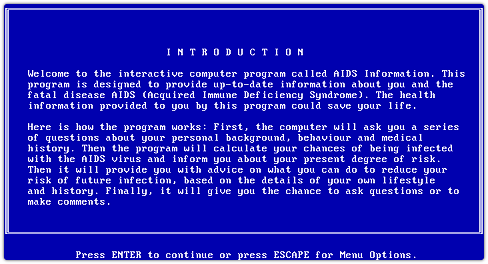
\includegraphics[width=\linewidth]{img/aids1.png}
		\caption{Lizenzvereinbarung AIDS \\ Quelle: \cite{aids:sophos}}
		\label{fig:lizenz_aids}
	\end{figure}

		Nach der Installation wurde mittels eines Zählers in der Autostart-Datei des Systems ermittelt, wie oft der Computer gestartet worden ist. War der 90. Start 
		erreicht, verschlüsselte der Virus die Namen von vordefinierten Dateien und Verzeichnissen, nicht aber deren Inhalt. Dies betraf auch wichtige Systemprogramme, die 
		ein Kommando-orientiertes Betriebssystem wie MS-DOS erst benutzbar machen. \\
		Zeitgleich wurde dem Opfer eine Nachricht gezeigt, mit den genauen Anweisungen, wie die vorgebliche Nutzungsgebühr an den Hersteller zu bezahlen sei. 
		Scheinbar legitimiert wird dieses Vorgehen mit den Lizenzvereinbarungen, die während der Installation vom Benutzer akzeptiert wurden. 

		Eine Analyse des Virus zeigte, dass vor allem die Verwendung einer symmetrischen Verschlüsselung (siehe Kapitel~\ref{sec:sym_verschl}). 
		Da hierfür die Schlüssel für die Ver- und Entschlüsselung gleich sind und prinzipbedingt im Virus selbst hinterlegt sein müssen, bot sich hier ein Angriffspunkt, um die
		Verschlüsselung auch ohne Zahlung der geforderten Geldsumme umzukehren. Erleichternd kommt hier dazu, dass die Schlüssel hart-codiert sind, und alle Infektionen
		den gleichen Schlüssel verwenden. \\
		So ist es nicht verwunderlich, dass sich bald Entschlüsselungswerkzeuge verbreiteten und damit die Wirkung des Virus außer Kraft setzten. \\
		Eine Untersuchung durch Adam Young und Moti Yung, schlug hier die Verwendung von asymmetrischer Verschlüsselung (siehe Kapitel~\ref{sec:asym_verschl}) vor, um einen
		Vorteil über das Opfer zu erhalten. \footcite{aids:young}
		
		Die Autoren heutiger Ransomware haben sich diesen Vorschlag zu Herzen genommen, sodass eine asymmetrische Verschlüsselung heute fast ausnahmslos in Ransomware 
		verwendet wird. Auch entscheidende Konzepte von AIDSinfo werden immer noch benutzt, sei des einen vorgeblichen Nutzen des Programms anzubieten oder auch nicht 
		direkt nach der Infektion aktiv zu werden, sondern noch einige Zeit abzuwarten. 

\section{Überblick über aktuelle Ransomware}
\label{sec:overview}
Locker / Locky / KeRanger ...

\section{Faktoren von Ransomware} 
	Ökonomie / Psychologie / Social-Engineering
	
\section{Überblick Verschlüsselung}
Dieses Kapitel soll eine kurze Einführung über Verschlüsselungen geben, allerdings wird hier im Rahmen der Lesbarkeit auf mathematische Exaktheit verzichtet. Ebenso werden
die einzelnen Punkte nur insoweit erklärt und beschrieben, wie für ein Verständnis über deren Anwendung in Rahmen von Ransomware notwendig ist. 

Für genauere Betrachtungen sei die einschlägige Fachliteratur hierüber empfohlen. % Beispiele
\subsection{Symmetrische Verschlüsselung}
\label{sec:sym_verschl}

Die symmetrische Verschlüsselung folgt dem Konzept, das sowohl für die Ver- als auch die Entschlüsselung jeweils die gleichen Schlüssel verwendet werden.
\afterpage{
\begin{figure}[h!]
	\centering
	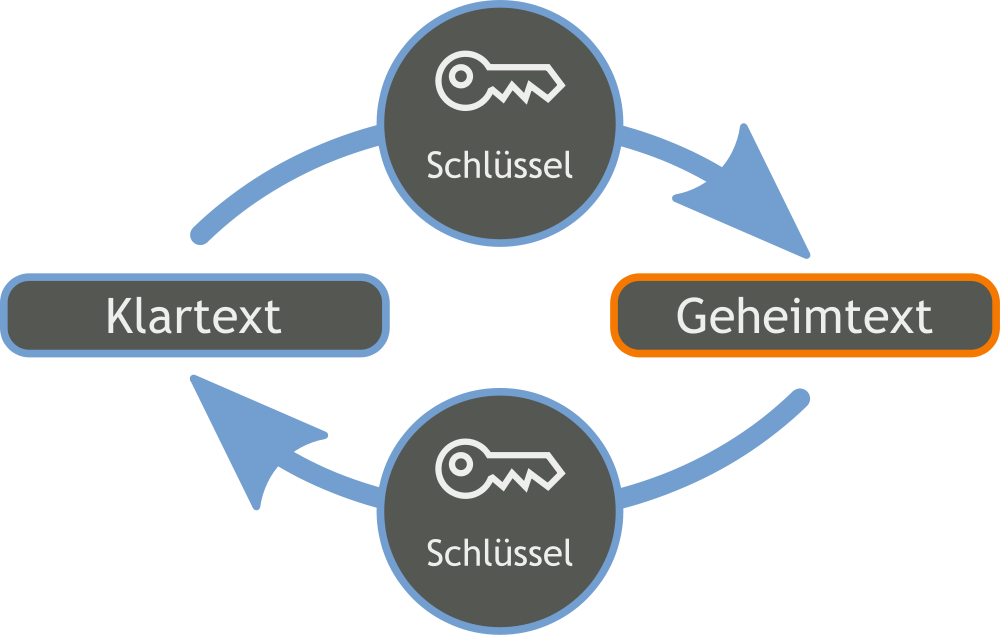
\includegraphics[width=\linewidth]{img/SymKrypto.png}
	\caption{Symmetrische Verschlüsselung mit identischen Schlüsseln\footnotemark}
	\label{fig:sym_verschl}
	\end{figure}
	\footnotetext{Quelle: Bananenfalter (Public Domain) \\ \url{https://commons.wikimedia.org/wiki/File:Orange_blue_symmetric_cryptography_de.svg}}
}
Es gibt eine Reihe an unterschiedlichsten Algorithmen und Verfahren für symmetrische Verschlüsselung, allerdings hat sich mit \textsc{AES} ein Verfahren als de-facto Standard für verschiedenste Anwendungsbereiche etabliert.

AES ist hierbei eine Abkürzung für Advanced Encryption Standard und wird meist synonym für den Rijndael-Algorithmus verwendet. Dieses Verfahren ist heute so verbreitet, dass beispielsweise in modernen Prozessoren direkt als Maschinenbefehl zur Verfügung steht und somit deutlich größere Datenraten verarbeiten kann. \\
Benchmarks zeigen hier beispielshaft einen 6-fachen Speedup mit einer Datenrate von ca. 1.35 GB/s mit CPU-Unterstützung verglichen mit 212 MB/s ohne 
CPU-Unterstützung.\footcite{aes:benchmark}

Vor allem durch die Hardware-Unterstützung ist es moderner Ransomware möglich, die CPU-Last während der Verschlüsselung derart in Grenzen zu halten, dass der Nutzer keine spürbare Langsamkeit des Systems bemerkt. 


\subsection{Asymmetrische Verschlüsselung}
\label{sec:asym_verschl}

\afterpage{
\begin{figure}[h!]
	\centering
	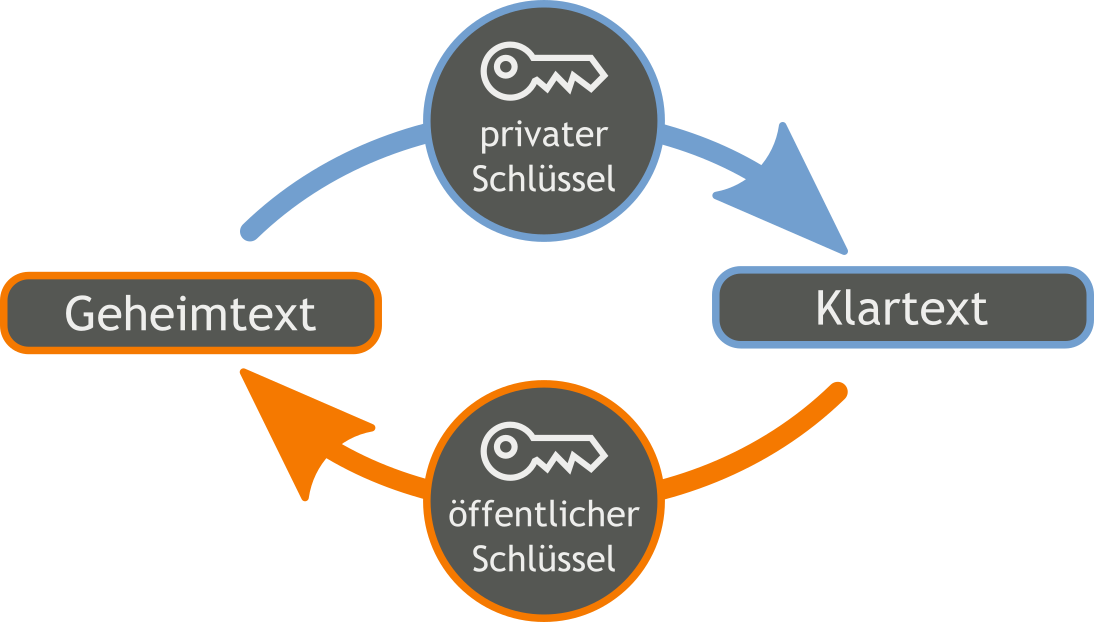
\includegraphics[width=\linewidth]{img/AsymKrypto.png}
	\caption{Asymmetrische Verschlüsselung\footnotemark}
	\label{fig:asym_verschl}
	\end{figure}
	\footnotetext{Quelle: Bananenfalter (Public Domain) \\ \url{https://commons.wikimedia.org/wiki/File:Orange_blue_symmetric_cryptography_de.svg}} %TODO: Url
}

Asymmetrische Verschlüsselung basiert auf zwei Schlüsseln, einen öffentlichen und einen privaten. Diese Schlüssel gehören mathematisch zusammen und werden für unterschiedliche Zwecke verwendet.
Soll ein Klartext verschlüsselt werden, so wird hierfür der öffentliche Schlüssel des Empfängers verwendet. Die Entschlüsselung muss dann mit dem zugehörigen privaten Schlüssel erfolgen, eine Entschlüsselung mit dem öffentlichen Schlüssel ist nicht mehr möglich.

Auf Grund der Komplexität der Berechnungen ist das Verfahren langsam und auch nur schwer in Hardware abzubilden. Deshalb wird es nur für verhältnismäßig kurze Klartexte verwendet (< 1 KB), auch da die maximale Länge des Klartexts von der Länge des verwendeten Schlüssels abhängt. %TODO: Nachweis


Der große Vorteil von asymmetrischer Verschlüsselung liegt im sicheren Schlüsselaustausch, der nicht auf einen bereits gesicherten Kanal angewiesen ist, sondern auch über ein unsicheres Medium, beispielsweise über das Internet erfolgen kann, ohne dass es für einen Angreifer möglich ist die beteiligten Schlüssel zu belauschen oder zu berechnen. %TODO: MitM




\subsection{Hybride Verschlüsselung}
\label{sec:hybride_verschl}

Hybride Verschlüsselung kombiniert alle Vorteile von symmetrischer Verschlüsselung (Geschwindigkeit, Einfachheit) mit allen Vorteilen von asymmetrischer Verschlüsselung (Schlüsseltausch, Sicherheit). 
Hierfür werden zufällige Schlüssel erzeugt, meist lange Zufallszahlen, die für die symmetrische Verschlüsselung verwendet werden. Diese Schlüssel werden Sitzungsschlüssel genannt und werden in der Regel nur einmalig verwendet (ein sog. One-Time-Pad). Nach der Verwendung werden die Sitzungsschlüssel asymmetrisch verschlüsselt und mit den codierten Daten zusammen übertragen.

Auf diese Weise lassen sich auch große Mengen an Daten effizient mittels asymmetrischer Kryptographie übertragen. 




\section{Überblick Anonyme Zahlungen}
Eine weitere Komponente warum heutige Ransomware so erfolgreich ist, stellt die Möglichkeit einer anonymen Bezahlung dar, vor allem in Hinsicht auf die Anonymität des Zahlungsempfängers. Hier stehen dem Angreifer verschiedene Zahlungsverfahren zur Auswahl, von eher traditioneller Überweisung bis hin zu Bitcoins.

\subsection{Ukash}
\subsection{Paysafecard}
\subsection{Western Union}
\subsection{Bitcoin}

\section{Überblick Tor-Netzwerk}
	Tor / Aufbau / Hidden Services / Anonymität

\section{Genereller Ablauf}
 CC Server / Verschlüsselung / Zahlung

\section{Weitere Beobachtungen}
Ransomware as a service

\section{Gegenmaßnahmen}
 
Backups / Heuristiken / Backups / Nutzerschulung / Backups / 

\section{Schluss}


